\documentclass[]{article}
\usepackage{lmodern}
\usepackage{amssymb,amsmath}
\usepackage{ifxetex,ifluatex}
\usepackage{fixltx2e} % provides \textsubscript
\ifnum 0\ifxetex 1\fi\ifluatex 1\fi=0 % if pdftex
  \usepackage[T1]{fontenc}
  \usepackage[utf8]{inputenc}
\else % if luatex or xelatex
  \ifxetex
    \usepackage{mathspec}
  \else
    \usepackage{fontspec}
  \fi
  \defaultfontfeatures{Ligatures=TeX,Scale=MatchLowercase}
    \setmainfont[]{Verdana}
    \setmonofont[Mapping=tex-ansi]{Consolas}
    \setmathfont(Digits,Latin,Greek)[]{Iwona}
\fi
% use upquote if available, for straight quotes in verbatim environments
\IfFileExists{upquote.sty}{\usepackage{upquote}}{}
% use microtype if available
\IfFileExists{microtype.sty}{%
\usepackage{microtype}
\UseMicrotypeSet[protrusion]{basicmath} % disable protrusion for tt fonts
}{}
\usepackage[margin=1in]{geometry}
\usepackage{hyperref}
\hypersetup{unicode=true,
            pdftitle={Abalone Reproductive Data},
            pdfauthor={Craig Mundy},
            pdfborder={0 0 0},
            breaklinks=true}
\urlstyle{same}  % don't use monospace font for urls
\usepackage{color}
\usepackage{fancyvrb}
\newcommand{\VerbBar}{|}
\newcommand{\VERB}{\Verb[commandchars=\\\{\}]}
\DefineVerbatimEnvironment{Highlighting}{Verbatim}{commandchars=\\\{\}}
% Add ',fontsize=\small' for more characters per line
\usepackage{framed}
\definecolor{shadecolor}{RGB}{248,248,248}
\newenvironment{Shaded}{\begin{snugshade}}{\end{snugshade}}
\newcommand{\AlertTok}[1]{\textcolor[rgb]{0.94,0.16,0.16}{#1}}
\newcommand{\AnnotationTok}[1]{\textcolor[rgb]{0.56,0.35,0.01}{\textbf{\textit{#1}}}}
\newcommand{\AttributeTok}[1]{\textcolor[rgb]{0.77,0.63,0.00}{#1}}
\newcommand{\BaseNTok}[1]{\textcolor[rgb]{0.00,0.00,0.81}{#1}}
\newcommand{\BuiltInTok}[1]{#1}
\newcommand{\CharTok}[1]{\textcolor[rgb]{0.31,0.60,0.02}{#1}}
\newcommand{\CommentTok}[1]{\textcolor[rgb]{0.56,0.35,0.01}{\textit{#1}}}
\newcommand{\CommentVarTok}[1]{\textcolor[rgb]{0.56,0.35,0.01}{\textbf{\textit{#1}}}}
\newcommand{\ConstantTok}[1]{\textcolor[rgb]{0.00,0.00,0.00}{#1}}
\newcommand{\ControlFlowTok}[1]{\textcolor[rgb]{0.13,0.29,0.53}{\textbf{#1}}}
\newcommand{\DataTypeTok}[1]{\textcolor[rgb]{0.13,0.29,0.53}{#1}}
\newcommand{\DecValTok}[1]{\textcolor[rgb]{0.00,0.00,0.81}{#1}}
\newcommand{\DocumentationTok}[1]{\textcolor[rgb]{0.56,0.35,0.01}{\textbf{\textit{#1}}}}
\newcommand{\ErrorTok}[1]{\textcolor[rgb]{0.64,0.00,0.00}{\textbf{#1}}}
\newcommand{\ExtensionTok}[1]{#1}
\newcommand{\FloatTok}[1]{\textcolor[rgb]{0.00,0.00,0.81}{#1}}
\newcommand{\FunctionTok}[1]{\textcolor[rgb]{0.00,0.00,0.00}{#1}}
\newcommand{\ImportTok}[1]{#1}
\newcommand{\InformationTok}[1]{\textcolor[rgb]{0.56,0.35,0.01}{\textbf{\textit{#1}}}}
\newcommand{\KeywordTok}[1]{\textcolor[rgb]{0.13,0.29,0.53}{\textbf{#1}}}
\newcommand{\NormalTok}[1]{#1}
\newcommand{\OperatorTok}[1]{\textcolor[rgb]{0.81,0.36,0.00}{\textbf{#1}}}
\newcommand{\OtherTok}[1]{\textcolor[rgb]{0.56,0.35,0.01}{#1}}
\newcommand{\PreprocessorTok}[1]{\textcolor[rgb]{0.56,0.35,0.01}{\textit{#1}}}
\newcommand{\RegionMarkerTok}[1]{#1}
\newcommand{\SpecialCharTok}[1]{\textcolor[rgb]{0.00,0.00,0.00}{#1}}
\newcommand{\SpecialStringTok}[1]{\textcolor[rgb]{0.31,0.60,0.02}{#1}}
\newcommand{\StringTok}[1]{\textcolor[rgb]{0.31,0.60,0.02}{#1}}
\newcommand{\VariableTok}[1]{\textcolor[rgb]{0.00,0.00,0.00}{#1}}
\newcommand{\VerbatimStringTok}[1]{\textcolor[rgb]{0.31,0.60,0.02}{#1}}
\newcommand{\WarningTok}[1]{\textcolor[rgb]{0.56,0.35,0.01}{\textbf{\textit{#1}}}}
\usepackage{graphicx,grffile}
\makeatletter
\def\maxwidth{\ifdim\Gin@nat@width>\linewidth\linewidth\else\Gin@nat@width\fi}
\def\maxheight{\ifdim\Gin@nat@height>\textheight\textheight\else\Gin@nat@height\fi}
\makeatother
% Scale images if necessary, so that they will not overflow the page
% margins by default, and it is still possible to overwrite the defaults
% using explicit options in \includegraphics[width, height, ...]{}
\setkeys{Gin}{width=\maxwidth,height=\maxheight,keepaspectratio}
\IfFileExists{parskip.sty}{%
\usepackage{parskip}
}{% else
\setlength{\parindent}{0pt}
\setlength{\parskip}{6pt plus 2pt minus 1pt}
}
\setlength{\emergencystretch}{3em}  % prevent overfull lines
\providecommand{\tightlist}{%
  \setlength{\itemsep}{0pt}\setlength{\parskip}{0pt}}
\setcounter{secnumdepth}{5}
% Redefines (sub)paragraphs to behave more like sections
\ifx\paragraph\undefined\else
\let\oldparagraph\paragraph
\renewcommand{\paragraph}[1]{\oldparagraph{#1}\mbox{}}
\fi
\ifx\subparagraph\undefined\else
\let\oldsubparagraph\subparagraph
\renewcommand{\subparagraph}[1]{\oldsubparagraph{#1}\mbox{}}
\fi

%%% Use protect on footnotes to avoid problems with footnotes in titles
\let\rmarkdownfootnote\footnote%
\def\footnote{\protect\rmarkdownfootnote}

%%% Change title format to be more compact
\usepackage{titling}

% Create subtitle command for use in maketitle
\providecommand{\subtitle}[1]{
  \posttitle{
    \begin{center}\large#1\end{center}
    }
}

\setlength{\droptitle}{-2em}

  \title{Abalone Reproductive Data}
    \pretitle{\vspace{\droptitle}\centering\huge}
  \posttitle{\par}
    \author{Craig Mundy}
    \preauthor{\centering\large\emph}
  \postauthor{\par}
      \predate{\centering\large\emph}
  \postdate{\par}
    \date{August 2018}

\usepackage{booktabs}
\usepackage{longtable}
\usepackage{array}
\usepackage{multirow}
\usepackage{wrapfig}
\usepackage{float}
\usepackage{colortbl}
\usepackage{pdflscape}
\usepackage{tabu}
\usepackage{threeparttable}
\usepackage{threeparttablex}
\usepackage[normalem]{ulem}
\usepackage{makecell}
\usepackage{xcolor}

\begin{document}
\maketitle

\begin{verbatim}
 [1] "channel"   "db.oocyte" "g3.g"      "g3.h"      "g3.oocyte" "g3.sf"     "sb.g"     
 [8] "sb.h"      "sb.sf"     "sql"       "sr.g"      "sr.h"      "sr.sf"    
\end{verbatim}

\hypertarget{the-project}{%
\section{The project}\label{the-project}}

Between 1988 and early 1992, Warwick Nash and team took monthly samples
(\textasciitilde{} 12 females) of abalone from George III Rock as part
of a study on spawning periodicity. During the last year of sampling
(1991), monthly samples were also taken at Shag Rock bay and Stinking
Bay on the Tasman Peninsular. Morphometric data were collected from each
animal, prior to the gonad being fixed. Routine histology was then done
on the gonads. The section was taken approximately 1/3 of the way along
the conical appendage on the basis that the gonad state was uniform
throughout.

Warwick Nash and team processed the histology slides, mapping out the
gonad state within the section into 8 categories. That work was never
published. In 2002, I (CM) had Leigh Gurney review the 8 state- gonad
classification system and re-classify the 8 states into a more typical 5
state system. Leigh also conducted detailed measureoments of oocyte
diameter for the 1991 Georges III Rock samples. Thi identfied a
transition from pre-vitellegenci to vitellegenic stages at around 95
microns. On the results of that exercise between 2004 and 2010 I had
various people process the histology slides for stage- frequency
analysis. The last person I employed casually was so efficient that I
ended up getting her to do the entire 4-year George III slides and the
slides from Shag Rock Bay and Stinking Bay, so that we had a consistent
dataset.

\hypertarget{the-data}{%
\subsection{The data}\label{the-data}}

The stage frequency data were collected from 4 transects across the
section oriented north, south, east, west. Within each transect the area
of the gonad sampled (outer membrane to boundary with the digestive
gland) was measured using imageJ, and a count done of the number of
pre-vitellegenic and vitellegenic oocytes in each transect.

Several data frames are loaded from this .R Data file. Sites are
designated as follows;

\begin{itemize}
\tightlist
\item
  g3.X = George III Rock
\item
  sr.X = Shag Rock Bay
\item
  sb.X = Stinking Bay
\end{itemize}

Different atasets are designated as follows;

\begin{itemize}
\tightlist
\item
  g3.g = basic morphometric information
\item
  g3.h = histology and gonad state information
\item
  g3.sf = stage frequency information
\end{itemize}

Examples are given below on joining the data frames to make a useable
dataset.

\hypertarget{gonad-data}{%
\subsection{Gonad data}\label{gonad-data}}

\begin{Shaded}
\begin{Highlighting}[]
\KeywordTok{kable}\NormalTok{(g3.g[}\DecValTok{1}\OperatorTok{:}\DecValTok{10}\NormalTok{,])}
\end{Highlighting}
\end{Shaded}

\begin{tabular}{r|r|l|r|r|r|r|r|l|r|r|r|r|r|r|r}
\hline
week\_no & abalone\_id & sample\_date & shell\_length\_mm & shell\_width\_mm & whole\_wt\_g & meat\_wt\_g & viscera\_wt\_g & sex & shell\_ht\_mm & shell\_wt\_g & no\_major\_rings & no\_minor\_rings & total\_no\_rings & samp\_year & samp\_month\\
\hline
1 & 7402 & 1988-02-11 & 132 & 101 & 334.4 & 158.8 & 82.8 & F & 42 & 80 & 13 & NA & 13 & 1988 & 2\\
\hline
1 & 7403 & 1988-02-11 & 140 & NA & 442.0 & 219.8 & 84.7 & M & NA & NA & NA & NA & NA & 1988 & 2\\
\hline
1 & 7404 & 1988-02-11 & 142 & 111 & 404.7 & 188.4 & 96.1 & F & 47 & 93 & 13 & NA & 13 & 1988 & 2\\
\hline
1 & 7405 & 1988-02-11 & 134 & NA & 363.6 & 179.7 & 85.9 & M & NA & NA & NA & NA & NA & 1988 & 2\\
\hline
1 & 7406 & 1988-02-11 & 117 & 92 & 195.2 & 93.0 & 35.2 & I & 30 & 54 & 13 & NA & 13 & 1988 & 2\\
\hline
1 & 7407 & 1988-02-11 & 136 & 115 & 390.4 & 170.7 & 83.4 & F & 41 & 104 & 14 & NA & 14 & 1988 & 2\\
\hline
1 & 7408 & 1988-02-11 & 97 & 79 & 136.1 & 61.0 & 30.1 & I & 25 & 36 & 6 & NA & 6 & 1988 & 2\\
\hline
1 & 7409 & 1988-02-11 & 132 & 107 & 380.5 & 189.5 & 82.3 & F & 33 & 87 & 14 & NA & 14 & 1988 & 2\\
\hline
1 & 7410 & 1988-02-11 & 126 & 99 & 293.9 & 146.7 & 54.0 & F & 35 & 71 & 10 & NA & 10 & 1988 & 2\\
\hline
1 & 7411 & 1988-02-11 & 123 & 93 & 190.5 & 80.7 & 40.5 & I & 31 & 57 & NA & NA & NA & 1988 & 2\\
\hline
\end{tabular}

\begin{Shaded}
\begin{Highlighting}[]
\KeywordTok{str}\NormalTok{(g3.g, }\DataTypeTok{digits.d =} \DecValTok{2}\NormalTok{, }\DataTypeTok{vec.len =} \DecValTok{3}\NormalTok{) }
\end{Highlighting}
\end{Shaded}

\begin{verbatim}
'data.frame':   3142 obs. of  16 variables:
 $ week_no        : num  1 1 1 1 1 1 1 1 ...
 $ abalone_id     : num  7402 7403 7404 7405 ...
 $ sample_date    : POSIXct, format: "1988-02-11" "1988-02-11" ...
 $ shell_length_mm: num  132 140 142 134 ...
 $ shell_width_mm : num  101 NA 111 NA ...
 $ whole_wt_g     : num  334 442 405 364 ...
 $ meat_wt_g      : num  159 220 188 180 ...
 $ viscera_wt_g   : num  83 85 96 86 ...
 $ sex            : Factor w/ 4 levels "F","I","M","T": 1 3 1 3 2 1 2 1 ...
 $ shell_ht_mm    : num  42 NA 47 NA 30 41 25 33 ...
 $ shell_wt_g     : num  80 NA 93 NA ...
 $ no_major_rings : num  13 NA 13 NA 13 14 6 14 ...
 $ no_minor_rings : num  NA NA NA NA NA NA NA NA ...
 $ total_no_rings : num  13 NA 13 NA 13 14 6 14 ...
 $ samp_year      : num  1988 1988 1988 1988 ...
 $ samp_month     : num  2 2 2 2 2 2 2 2 ...
\end{verbatim}

\hypertarget{histology-data}{%
\subsection{Histology data}\label{histology-data}}

\begin{Shaded}
\begin{Highlighting}[]
\KeywordTok{kable}\NormalTok{(g3.h[}\DecValTok{1}\OperatorTok{:}\DecValTok{10}\NormalTok{,])}
\end{Highlighting}
\end{Shaded}

\begin{tabular}{r|r|r|r|r|r|r|r|r|r|r|r|r|r|r|r|r|r|r|r|r|r|r|r|r|r|r|r|r|r}
\hline
week\_no & abalone\_id & shell\_length\_mm & whole\_wt\_g & no\_major\_rings & stage\_1\_mm2 & stage\_2\_mm2 & stage\_3\_mm2 & stage\_4\_mm2 & stage\_5\_mm2 & stage\_6\_mm2 & stage\_7\_mm2 & stage\_8\_mm2 & liver\_area\_mm2 & gonad\_area\_mm2 & gonad\_index & tafi\_index & pc\_developing & pc\_ripe & pc\_spent & rec\_dev & locules & mature & spawning & necrotic & pc\_rec\_dev & pc\_locules & pc\_mature & pc\_spawning & pc\_necrotic\\
\hline
1 & 7402 & 132 & 334.4 & 13 & 0.00 & 0.00 & 21.00 & 1.36 & 0.00 & 0.84 & 16.70 & 0.00 & 113.58 & 39.90 & 0.2599687 & 0 & 0.000 & 56.04010 & 43.9598997 & 0 & 21 & 1 & 17 & 1 & 0 & 53 & 3 & 43 & 3\\
\hline
1 & 7404 & 142 & 404.7 & 13 & 0.00 & 0.00 & 0.00 & 103.64 & 0.00 & 2.27 & 9.76 & 0.00 & 140.90 & 115.67 & 0.4508321 & 0 & 0.000 & 89.59972 & 10.4002766 & 0 & 0 & 104 & 10 & 2 & 0 & 0 & 90 & 9 & 2\\
\hline
1 & 7407 & 136 & 390.4 & 14 & 0.00 & 0.00 & 0.00 & 86.30 & 0.00 & 6.92 & 25.30 & 0.00 & 80.18 & 118.52 & 0.5964771 & 0 & 0.000 & 72.81471 & 27.1852852 & 0 & 0 & 86 & 25 & 7 & 0 & 0 & 73 & 21 & 6\\
\hline
1 & 7409 & 132 & 380.5 & 14 & 0.00 & 30.37 & 0.00 & 0.00 & 0.00 & 0.00 & 6.92 & 2.67 & 105.58 & 39.96 & 0.2745637 & 0 & 76.001 & 0.00000 & 23.9989990 & 33 & 0 & 0 & 7 & 0 & 83 & 0 & 0 & 18 & 0\\
\hline
1 & 7410 & 126 & 293.9 & 10 & 0.00 & 0.00 & 42.22 & 0.00 & 0.00 & 0.00 & 6.75 & 0.00 & 95.43 & 48.97 & 0.3391274 & 0 & 0.000 & 86.21605 & 13.7839494 & 0 & 42 & 0 & 7 & 0 & 0 & 86 & 0 & 14 & 0\\
\hline
1 & 7414 & 147 & 504.1 & 12 & 0.00 & 0.00 & 0.00 & 214.76 & 0.00 & 0.00 & 0.00 & 0.00 & 84.84 & 214.76 & 0.7168224 & 0 & 0.000 & 100.00000 & 0.0000000 & 0 & 0 & 215 & 0 & 0 & 0 & 0 & 100 & 0 & 0\\
\hline
1 & 7415 & 138 & 348.2 & 12 & 17.04 & 0.00 & 0.00 & 0.00 & 0.00 & 0.00 & 0.00 & 0.00 & 135.67 & 17.04 & 0.1115840 & 0 & 100.000 & 0.00000 & 0.0000000 & 17 & 0 & 0 & 0 & 0 & 100 & 0 & 0 & 0 & 0\\
\hline
1 & 7416 & 125 & 278.8 & 9 & 0.00 & 0.00 & 61.95 & 0.00 & 0.00 & 0.00 & 6.09 & 0.00 & 163.28 & 68.04 & 0.2941380 & 0 & 0.000 & 91.04938 & 8.9506173 & 0 & 62 & 0 & 6 & 0 & 0 & 91 & 0 & 9 & 0\\
\hline
1 & 7417 & 158 & 649.6 & 14 & 0.00 & 0.00 & 129.55 & 0.00 & 0.00 & 0.00 & 24.28 & 0.00 & 162.91 & 153.83 & 0.4856665 & 0 & 0.000 & 84.21634 & 15.7836573 & 0 & 130 & 0 & 24 & 0 & 0 & 85 & 0 & 16 & 0\\
\hline
1 & 7418 & 134 & 384.7 & 14 & 0.00 & 0.00 & 0.00 & 240.65 & 50.02 & 2.42 & 0.00 & 0.00 & 112.39 & 293.09 & 0.7228223 & 0 & 0.000 & 99.17432 & 0.8256849 & 0 & 0 & 291 & 0 & 2 & 0 & 0 & 99 & 0 & 1\\
\hline
\end{tabular}

\begin{Shaded}
\begin{Highlighting}[]
\KeywordTok{str}\NormalTok{(g3.h, }\DataTypeTok{digits.d =} \DecValTok{2}\NormalTok{, }\DataTypeTok{vec.len =} \DecValTok{3}\NormalTok{) }
\end{Highlighting}
\end{Shaded}

\begin{verbatim}
'data.frame':   746 obs. of  30 variables:
 $ week_no        : num  1 1 1 1 1 1 1 1 ...
 $ abalone_id     : num  7402 7404 7407 7409 ...
 $ shell_length_mm: num  132 142 136 132 ...
 $ whole_wt_g     : num  334 405 390 380 ...
 $ no_major_rings : num  13 13 14 14 10 12 12 9 ...
 $ stage_1_mm2    : num  0 0 0 0 ...
 $ stage_2_mm2    : num  0 0 0 30 ...
 $ stage_3_mm2    : num  21 0 0 0 ...
 $ stage_4_mm2    : num  1.4 103.6 86.3 0 ...
 $ stage_5_mm2    : num  0 0 0 0 0 0 0 0 ...
 $ stage_6_mm2    : num  0.84 2.27 6.92 0 ...
 $ stage_7_mm2    : num  16.7 9.8 25.3 6.9 ...
 $ stage_8_mm2    : num  0 0 0 2.7 ...
 $ liver_area_mm2 : num  114 141 80 106 ...
 $ gonad_area_mm2 : num  40 116 119 40 ...
 $ gonad_index    : num  0.26 0.45 0.6 0.27 ...
 $ tafi_index     : num  0 0 0 0 0 0 0 0 ...
 $ pc_developing  : num  0 0 0 76 ...
 $ pc_ripe        : num  56 90 73 0 ...
 $ pc_spent       : num  44 10 27 24 ...
 $ rec_dev        : int  0 0 0 33 0 0 17 0 ...
 $ locules        : int  21 0 0 0 42 0 0 62 ...
 $ mature         : int  1 104 86 0 0 215 0 0 ...
 $ spawning       : int  17 10 25 7 7 0 0 6 ...
 $ necrotic       : int  1 2 7 0 0 0 0 0 ...
 $ pc_rec_dev     : int  0 0 0 83 0 0 100 0 ...
 $ pc_locules     : int  53 0 0 0 86 0 0 91 ...
 $ pc_mature      : int  3 90 73 0 0 100 0 0 ...
 $ pc_spawning    : int  43 9 21 18 14 0 0 9 ...
 $ pc_necrotic    : int  3 2 6 0 0 0 0 0 ...
\end{verbatim}

\hypertarget{stage-frequency-data}{%
\subsection{Stage Frequency data}\label{stage-frequency-data}}

\begin{Shaded}
\begin{Highlighting}[]
\KeywordTok{kable}\NormalTok{(g3.sf[}\DecValTok{1}\OperatorTok{:}\DecValTok{10}\NormalTok{,])}
\end{Highlighting}
\end{Shaded}

\begin{tabular}{l|l|r|r|r|l|r|r|r}
\hline
site & sample\_date & samp\_year & samp\_month & abalone\_id & quadrant & previt & vit & qarea\\
\hline
G3R & 1988-09-09 & 1988 & 9 & 36022 & E & 102 & 1 & 0.359\\
\hline
G3R & 1988-09-09 & 1988 & 9 & 36022 & N & 0 & 0 & 0.000\\
\hline
G3R & 1988-09-09 & 1988 & 9 & 36022 & S & 68 & 2 & 0.577\\
\hline
G3R & 1988-09-09 & 1988 & 9 & 36022 & W & 72 & 4 & 0.324\\
\hline
G3R & 1988-09-09 & 1988 & 9 & 36032 & E & 37 & 10 & 0.954\\
\hline
G3R & 1988-09-09 & 1988 & 9 & 36032 & N & 13 & 4 & 1.287\\
\hline
G3R & 1988-09-09 & 1988 & 9 & 36032 & S & 79 & 5 & 2.832\\
\hline
G3R & 1988-09-09 & 1988 & 9 & 36032 & W & 141 & 17 & 3.498\\
\hline
G3R & 1988-09-09 & 1988 & 9 & 36033 & E & 83 & 41 & 1.908\\
\hline
G3R & 1988-09-09 & 1988 & 9 & 36033 & N & 35 & 33 & 2.280\\
\hline
\end{tabular}

\begin{Shaded}
\begin{Highlighting}[]
\KeywordTok{str}\NormalTok{(g3.sf, }\DataTypeTok{digits.d =} \DecValTok{2}\NormalTok{, }\DataTypeTok{vec.len =} \DecValTok{3}\NormalTok{) }
\end{Highlighting}
\end{Shaded}

\begin{verbatim}
'data.frame':   2223 obs. of  9 variables:
 $ site       : Factor w/ 1 level "G3R": 1 1 1 1 1 1 1 1 ...
 $ sample_date: POSIXct, format: "1988-09-09" "1988-09-09" ...
 $ samp_year  : num  1988 1988 1988 1988 ...
 $ samp_month : num  9 9 9 9 9 9 9 9 ...
 $ abalone_id : num  36022 36022 36022 36022 ...
 $ quadrant   : Factor w/ 4 levels "E","N","S","W": 1 2 3 4 1 2 3 4 ...
 $ previt     : num  102 0 68 72 ...
 $ vit        : num  1 0 2 4 10 4 5 17 ...
 $ qarea      : num  0.36 0 0.58 0.32 ...
\end{verbatim}

\hypertarget{joining-the-tables}{%
\section{Joining the tables}\label{joining-the-tables}}

\hypertarget{morphometrics-and-histology}{%
\subsection{Morphometrics and
Histology}\label{morphometrics-and-histology}}

\begin{Shaded}
\begin{Highlighting}[]
\CommentTok{## Add histology data to morpomeric data }
\NormalTok{histodat <-}\StringTok{ }\KeywordTok{left_join}\NormalTok{(g3.g, g3.h ) }\OperatorTok\StringTok{ }
\StringTok{ }\KeywordTok{filter}\NormalTok{(}\OperatorTok{!}\KeywordTok{is.na}\NormalTok{(tafi_index)) }\OperatorTok\StringTok{ }
\StringTok{ }\KeywordTok{ungroup}\NormalTok{()}
\end{Highlighting}
\end{Shaded}

\begin{verbatim}
Joining, by = c("week_no", "abalone_id", "shell_length_mm", "whole_wt_g", "no_major_rings")
\end{verbatim}

\begin{Shaded}
\begin{Highlighting}[]
\NormalTok{histodat }\OperatorTok\StringTok{ }\KeywordTok{filter}\NormalTok{(sex }\OperatorTok{==}\StringTok{ "F"}\NormalTok{ ) }\OperatorTok\StringTok{ }
\StringTok{ }\KeywordTok{group_by}\NormalTok{(samp_year, samp_month) }\OperatorTok
\StringTok{ }\KeywordTok{summarise}\NormalTok{(}\DataTypeTok{reps =} \KeywordTok{n}\NormalTok{()) }\OperatorTok\StringTok{ }\KeywordTok{kable}\NormalTok{()}
\end{Highlighting}
\end{Shaded}

\begin{tabular}{r|r|r}
\hline
samp\_year & samp\_month & reps\\
\hline
1988 & 2 & 15\\
\hline
1988 & 3 & 13\\
\hline
1988 & 4 & 9\\
\hline
1988 & 5 & 9\\
\hline
1988 & 7 & 13\\
\hline
1988 & 8 & 13\\
\hline
1988 & 9 & 13\\
\hline
1988 & 10 & 12\\
\hline
1988 & 11 & 13\\
\hline
1988 & 12 & 11\\
\hline
1989 & 1 & 14\\
\hline
1989 & 2 & 12\\
\hline
1989 & 5 & 7\\
\hline
1989 & 6 & 13\\
\hline
1989 & 7 & 14\\
\hline
1989 & 9 & 18\\
\hline
1989 & 10 & 4\\
\hline
1989 & 12 & 2\\
\hline
1990 & 1 & 1\\
\hline
1990 & 2 & 12\\
\hline
1990 & 3 & 6\\
\hline
1990 & 4 & 14\\
\hline
1990 & 5 & 11\\
\hline
1990 & 6 & 11\\
\hline
1990 & 7 & 15\\
\hline
1990 & 8 & 19\\
\hline
1990 & 9 & 15\\
\hline
1990 & 10 & 17\\
\hline
1990 & 11 & 16\\
\hline
1990 & 12 & 13\\
\hline
1991 & 1 & 15\\
\hline
1991 & 2 & 15\\
\hline
1991 & 3 & 16\\
\hline
1991 & 4 & 14\\
\hline
1991 & 5 & 14\\
\hline
1991 & 6 & 12\\
\hline
1991 & 7 & 12\\
\hline
1991 & 8 & 16\\
\hline
1991 & 9 & 13\\
\hline
1991 & 10 & 18\\
\hline
1991 & 11 & 17\\
\hline
1991 & 12 & 19\\
\hline
1992 & 1 & 16\\
\hline
\end{tabular}

\hypertarget{morphometrics-and-histology-1}{%
\subsection{Morphometrics and
Histology}\label{morphometrics-and-histology-1}}

Not all histology slides were processed for stage frequency. Some
sections were too fragmented or of poor quality, and were skipped.

\begin{Shaded}
\begin{Highlighting}[]
\CommentTok{## first step is to summarise the data in each transect}
\NormalTok{g3sfdat <-}\StringTok{ }\NormalTok{g3.sf }\OperatorTok\StringTok{ }\KeywordTok{filter}\NormalTok{(qarea }\OperatorTok{>}\StringTok{ }\DecValTok{0}\NormalTok{) }\OperatorTok\StringTok{ }
\StringTok{  }\KeywordTok{group_by}\NormalTok{(abalone_id) }\OperatorTok\StringTok{ }
\StringTok{  }\KeywordTok{summarise}\NormalTok{(}\DataTypeTok{vits =} \KeywordTok{sum}\NormalTok{(vit, }\DataTypeTok{na.rm=}\NormalTok{T),}
            \DataTypeTok{previts =} \KeywordTok{sum}\NormalTok{(previt, }\DataTypeTok{na.rm=}\NormalTok{T),}
            \DataTypeTok{sum_area =} \KeywordTok{sum}\NormalTok{(qarea, }\DataTypeTok{na.rm=}\NormalTok{T),}
            \DataTypeTok{ntrans =} \KeywordTok{n}\NormalTok{())}

\CommentTok{## Add summarised stage frequency data to histo and morphometric data }
\NormalTok{stagedat <-}\StringTok{ }\KeywordTok{left_join}\NormalTok{(histodat, g3sfdat ) }\OperatorTok\StringTok{ }
\StringTok{ }\KeywordTok{ungroup}\NormalTok{()}
\end{Highlighting}
\end{Shaded}

\begin{verbatim}
Joining, by = "abalone_id"
\end{verbatim}

\hypertarget{simple-stage-frequency-plots}{%
\subsection{simple stage frequency
plots}\label{simple-stage-frequency-plots}}

Some basic plots of the relationship between shell length and the number
of vits and previts, colour coded by month, and with a bubble size set
by the section area sampled.

\begin{Shaded}
\begin{Highlighting}[]
\NormalTok{stagedat }\OperatorTok\StringTok{ }\KeywordTok{ggplot}\NormalTok{(}\KeywordTok{aes}\NormalTok{(}\DataTypeTok{x=}\NormalTok{shell_length_mm, }\DataTypeTok{y=}\NormalTok{vits, }\DataTypeTok{colour=}\NormalTok{samp_month, }\DataTypeTok{size =}\NormalTok{ sum_area)) }\OperatorTok{+}
\KeywordTok{geom_point}\NormalTok{(}\DataTypeTok{alpha =} \FloatTok{0.9}\NormalTok{)}
\end{Highlighting}
\end{Shaded}

\begin{verbatim}
Warning: Removed 138 rows containing missing values (geom_point).
\end{verbatim}

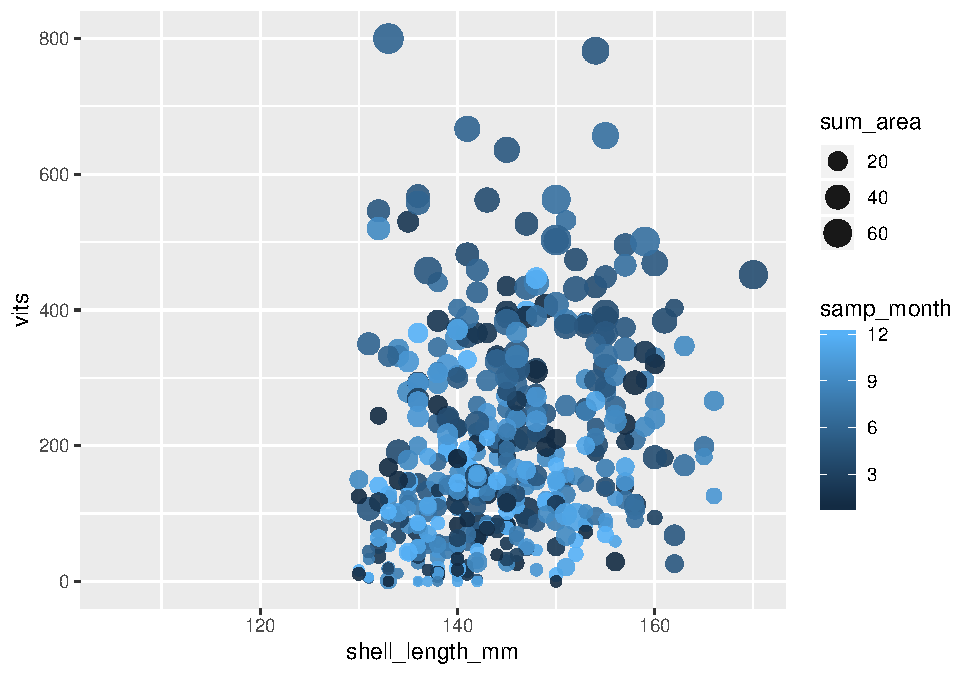
\includegraphics{AbRepro_files/figure-latex/simple plots-1.pdf}

\begin{Shaded}
\begin{Highlighting}[]
\NormalTok{stagedat }\OperatorTok\StringTok{ }\KeywordTok{ggplot}\NormalTok{(}\KeywordTok{aes}\NormalTok{(}\DataTypeTok{x=}\NormalTok{shell_length_mm, }\DataTypeTok{y=}\NormalTok{previts, }\DataTypeTok{colour=}\NormalTok{samp_month, }\DataTypeTok{size =}\NormalTok{ sum_area)) }\OperatorTok{+}
\KeywordTok{geom_point}\NormalTok{(}\DataTypeTok{alpha =} \FloatTok{0.9}\NormalTok{)}
\end{Highlighting}
\end{Shaded}

\begin{verbatim}
Warning: Removed 138 rows containing missing values (geom_point).
\end{verbatim}

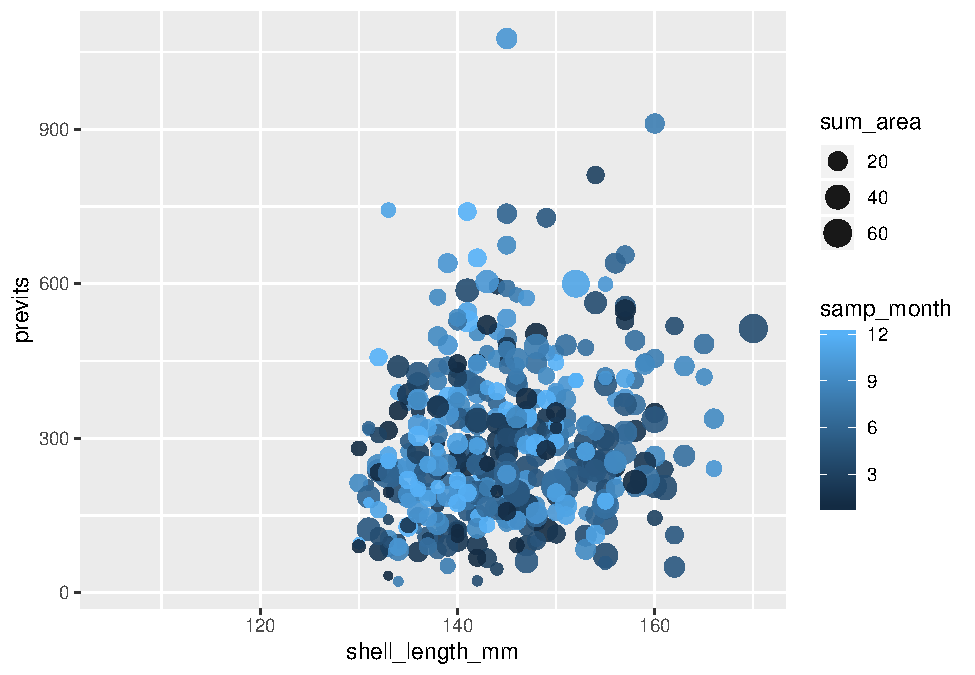
\includegraphics{AbRepro_files/figure-latex/simple plots-2.pdf}


\end{document}
